\documentclass[fleqn,10pt]{wlscirep} 

\usepackage{setspace}
\usepackage{lineno}
\doublespacing


%%%% (20 words or less)
\title{Genotypic variation in a foundation tree drives ecological network structure}

\author[1,2,*]{Matthew K. Lau}
\author[2]{Louis J. Lamit}
\author[3]{Rikke R. Naesbourg}
\author[4]{Stuart R. Borrett}
\author[5]{Matthew A. Bowker}
\author[1]{Thomas G. Whitham}

\affil[1]{Department of Biological Sciences and Merriam-Powell Center
  for Environmental Research, Northern Arizona University, Flagstaff,
  AZ 86011, USA}
\affil[2]{Harvard Forest, Harvard University, 324 N Main St,
  Petersham, MA 01366, USA}
\affil[3]{University of California Berkeley, Berkeley, CA, USA}
\affil[4]{Department of Biology and Marine Biology, University of
  North Carolina Wilmington, 601 South College Road, Wilmington, NC,
  28403, USA}
\affil[5]{School of Forestry, Northern Arizona University, Flagstaff,
  AZ 86011, USA}

\affil[*]{matthewklau@fas.harvard.edu}

%% \affil[+]{these authors contributed equally to this work}

\keywords{Keyword1, Keyword2, Keyword3}

\begin{abstract}

Biological evolution occurs in the context of complex networks of
interacting species in which natural selection defines the structure
of ecological networks. Fundamental to this evolutionary process is
the discovery of a genetic basis to ecological network
structure. Although previous work has demonstrated that tree genotype
contributes to interaction network structure at the scale of forest
stands, the contribution of tree genetics to localized interaction
networks at the scale of individual trees has not yet been
explored. To test the degree to which tree genetics can contribute to
network structure across scales from trees to stands, we conducted
quantitative modeling of interaction network for a community of
epiphytic lichens in a long-term experimental common garden of
genotyped trees of a foundation species (\textit{Populus
  angustifolia}). We found three main results: 1) Tree genotype
strongly contributed to network structure explaining over a third of
the variation in lichen interaction networks, 2) Multiple aspects of
interaction network structure varied in response to genotype,
including network size, the number of interactions, linkage density
and connectance, 3) At the stand scale, we also found signficant
modular structure of plant-lichen networks resulting in part from the
combination of trees of the same genotype tending to have similar
community compositions and supporting similar lichen interaction
networks dominated by positive interactions. These results support the
hypothesis that variation in ecological interaction networks can
result from genetically based variation in foundation
species. Although these results are for a community of sessile
organisms in close proximity to the tree, this study opens the
possibility for a genetic basis to both direct and indirect
interactions among species in complex communities.

\end{abstract}

\begin{document}

\flushbottom
\maketitle
% * <john.hammersley@gmail.com> 2015-02-09T12:07:31.197Z:
%
%  Click the title above to edit the author information and abstract
%
% ^ <thomas.whitham@nau.edu> 2018-03-02T21:05:44.603Z.
\thispagestyle{empty}

%% \noindent Please note: Abbreviations should be introduced at the
%% first mention in the main text – no abbreviations lists. Suggested
%% structure of main text (not enforced) is provided below.

\linenumbers

%%% For Submission to Nature Ecology and Evolution %%%
%%% https://www.nature.com/natecolevol/info


\section*{Introduction}

Evolution occurs in the context of complex networks of interacting
species. In ecological communities, community dynamics depend on key
interactions \cite{Fontaine2011} that occur in species interaction
networks, such as:  trophic \cite{Bascompte2006} and mutualistic
\cite{Rafferty2013} interaction networks. Phylogenetic patterns in
ecological networks support the importance of evolutionary processes
in shaping species interactions, community structure and ecosystem
processes \cite{Crutsinger 2016, Rezende2007, Whitham2006a}. Community
genetics studies \cite{Lamit et al. 2015} have shown that genetic
variation in foundation species \cite{Ellison2005} plays a significant
role in defining distinct communities of interacting organisms:  such
as, endophytes, pathogens, lichens, arthropods, and soil
microbes. Multiple studies have now demonstrated that genetic
variation influences numerous functional traits (e.g., phytochemical,
phenological, morphological) produces a multivariate phenotype
\cite{holeski2012} tha contributes to variation in associated
communities \cite{Bailey2009a}. 


Additional work has provided support for the hypothesis that not only
does composition vary among genetically distinct genotypes of
foundation species but it also impacts the structure of the network of
species interactions in these communities \cite{Keith2017,
  Lau2016}. Also, work by \citep{Toju 2018, Toju2015, Toju2014}
observed consistent patterns of centralized interactions of species
modules focused around hubs of plant-fungal interactions. In other
words, a small number of plant and fungal symbionts tended to have
have disproportionate numbers of interactions with other species and
likely are the drivers in determining community assembly, structure
and dynamics.


\textbf{Foundation species, by defention, have large effects on ecosystems and
the networks of interacting species that make up the biotic component}

\cite{Thompson1999, Rowntree2011, DesRoches2017}
\citep{Ellison2005}
\cite{Martinsen2001}
\cite{Lamit2011}

Barbour2009

Ghering2017 

Lamit2016

Hughes?

Leroy?

Busby2015

Crutsinger2016

\textbf{Network structure is important for evolutionary dynamics}

\cite{Rezende2007, Guimaraes2011, Moya-Larano2011, Thompson2014, Fortin2017}



Bascompte2003

Rezende2007

Andreazzi2017

Toju2017

Dáttilo2016

\textbf{Networks found to ge generally stable through time and space}

Datillo2013

Díaz-Castelazo2010

Guimarães2007

Guimarães2006


\textbf{Genetic basis of networks}

Jormalainen2017

Fortuna et al. 2009

Solance2015

Lau2015

Lau2016

Keith2017


\textbf{None of the community genetics network papers have looked at
species-species newtorks of associated organisms at the scale of
individual tree genotypes}

Here, we investigate how genetic variation in a foundation tree
species determines the structure of a network of interactions among a
community of lichen species. Using a long-term (20 years+), common
garden experiment with replicated individuals of known genetic
identity and a naturally established stand of
\textit{P. angustifolia}. We focused on a model community of 9
epiphytic lichens species, as previous research has demonstrated
significant compositional responses of epiphytes to genotypic
variation \cite{Winfree2011, Zytynska2011}. In addition, the
life-history characteristics of lichen, having highly localized,
direct contact interactions and slow population turnover rates,
allowed us to assess interactions among lichen species on individual
trees. We hypothesize that in natural systems evolution occurs in a
community context involving interactions of complex networks of
interacting species \cite{Lau2016, Keith2017, Thompson2013,
  Bascompte2007, Darwin1855}.  If correct, we should expect to find
that network structure is genetically based in which different plant
genotypes support different interaction networks and that these
interactions networks can function as indicators of ecological
dynamics important for conserving biodiversity.  Applying a dual-scale
(lichen-lichen and genotype-lichen interactions) network modeling and
analyses, we then examined the genetically based impacts of
\textit{P. angustifolia} on network structure.

%% Topical subheadings are allowed. Authors must ensure that their
%% Methods section includes adequate experimental and characterization
%% data necessary for others in the field to reproduce their work.

\section*{Methods}

\subsection*{Field observations in common garden and natural riparian
  forest stands}

The study was conducted along the Weber River, UT (USA), which is a
cottonwood (\textit{Populus} spp.) dominated riparian
ecosystem. Although two native species, \textit{Populus angustifolia}
(James) and \textit{Populus fremontii} (S. Watson), occur here and are
known to hybridize, only pure or advanced generation backcrosses of
\textit{P. angustifolia} were sampled in order to avoid the effect of
the hybridization between these two species.

A common garden was used to isolate the effect of tree genotype from
the effect of the localized microenvironment associated with each
individual and spatial autocorrelation. Asexually propagated clones of
genotyped \textit{P. angustifolia} individuals4 were obtained from
wild collections and planted randomly in a single field (0.025 km$^2$)
at the Ogden Nature Center, Ogden, UT in 1992. A total of thirteen
genotypes replicated between 3 and 8 times each, were chosen for
sampling. Genotype names were previously published
\cite{Martinsen}. Observations were made in the common garden in
October 2010 and May 2011.

The natural stand of \textit{P. angustifolia} near the city of Uintah,
UT (GPS:  N41.13903, W110.94400) was used for the wild stand
survey. We conducted sampling of the stand in May 2012. A total of 14
trees were chosen randomly over a 0.10 km$^2$ area with a minimal
distance of 5.56 m between trees across a range of tree core based
ages from 15 to 60 years.

\subsection*{Bark and Lichen Community Observations}

On each tree, presence or absence of each lichen species was assessed
in 50 total 1 cm$^2$ cells arrayed in a checkerboard pattern. Two
adjacent 10 cm$^2$ quadrats centered at 50 cm and 85 cm from ground
level were sampled. The checkerboard sampling pattern was chosen to
isolate each cell based on an average thallus size of 1
cm$^2$. Samples were restricted to the northern aspect of the trunk to
maximize the abundance of lichen and control for the effect of
aspect. The thalli in each cell are expected to be spatially
independent of the other cells in the quadrat, but exposed to similar
micro-environmental conditions. Bark roughness was measured on each
tree following \cite{Winfree2011}.

The bark lichen community in this system is comprised of fourteen
species; however, only 9 species were observed within our study
quadrats. The lichen community included (abbreviations are given for
species present in study): Xg = \textit{Xanthomendoza galericulata},
Xm = \textit{X. montana}, Ch = \textit{Caloplaca holocarpa}, Cs =
\textit{Candelariella subdeflexa}, Rg = \textit{Rinodina glauca}, Lh =
\textit{Lecanora hagenii}, Ls = \textit{Lecanora} (unknown species),
Pm = \textit{Phyciella melanchra}, Pa = \textit{Physcia adscendens},
Pu = \textit{Physcia undulata}, \textit{Phaeophyscia orbicularis},
\textit{Phaeophyscia ciliata}, \textit{Melanelia subolivacea},
\textit{Meanelia elegantula}, including both crustose and foliose
lichen species that exhibit low inter-annual variation
\cite{Lamit2011}. We were able to rapidly assess lichen interactions
by quantifying thalli in closed contact as assessed using 1 cm$^2$
cells. Species accumulation curves showed that communities in the wild
and the common garden were thoroughly sampled and with similar species
richness (Supplementary Materials, Fig 1).


\subsection*{Network modeling and analyses}

We used the observations of lichen in the 1cm$^2$ cells on individual
trees of \textit{P. angustifolia} both in the common garden and the
natural stand. Uni-partite networks were generated using an analytical
procedure that removes non-significant interactions between species
\cite{Araujo2011}. In brief, the approach begins by calculating the
co-occurrences of all species pairs using the replicate cells. The
signficance of each interaction pair is determined by comparing the
observed frequency of co-occurrence to a theoretical ``null'' level of
co-occurrence.



\subsection*{Data and Analytical Software Availability}

All analyses were conducted using the R statistical programming
language \cite{RCoreTeam2017}. Code for the analyses is available on
github and data are available at Figshare.


\section*{Results}

%%% Up to three levels of \textbf{subheading} are permitted. Subheadings should not be numbered.

\subsection*{Tree Genotype Influences Ecological Network Structure}


\begin{figure}[ht]
\centering
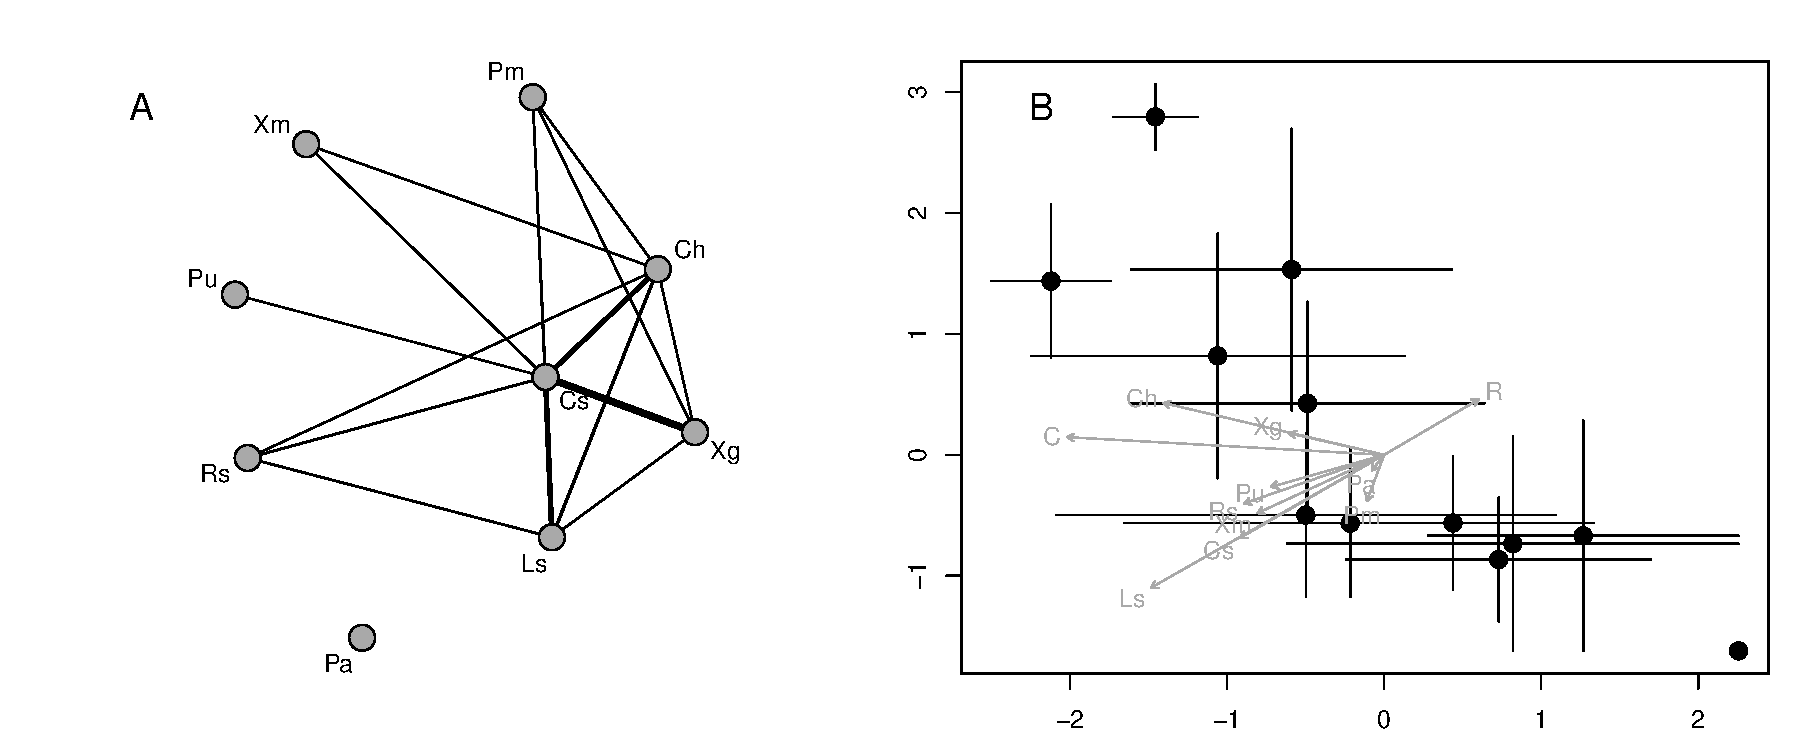
\includegraphics[width=\linewidth]{cn_chplot_onc.pdf}
\caption{Significant lichen interaction network structure resulting
  from tree genotypic variation was observed in the common garden. A)
  A network diagram showing significant interactions averaged over all
  trees shown as edges connecting lichen species shown as vertices. B)
  Genotype centroids (points) of NMDS ordinated lichen networks ($\pm$
  1 S.E.). Arrows show the magnitude and direction of correlation of
  the ordinated networks with tree bark roughness (R), network
  connectance and lichen species abundances (Xg =
  \textit{Xanthomendoza galericulata}, Xm = \textit{X. montana}, Ch =
  \textit{Caloplaca holocarpa}, Cs = \textit{Candelariella
    subdeflexa}, Rs = \textit{Rinodina} (unknown species), Ls =
  \textit{Lecanora} (unknown species), Pm = \textit{Phyciella
    melanchra}, Pa = \textit{Physcia adscendens}, Pu = \textit{Physcia
    undulata}).}
\label{fig:ch_plot}
\end{figure}

% latex table generated in R 3.4.4 by xtable 1.8-2 package
% Tue Sep 11 21:15:20 2018
\begin{table}[ht]
\centering
\begin{tabular}{lrrrrrr}
  \hline
 & Df & SumsOfSqs & MeanSqs & F.Model & R2 & Pr($>$F) \\ 
  \hline
onc.geno & 12.00000 & 163.74158 & 13.64513 & 1.87165 & 0.33795 & 0.04100 \\ 
  Residuals & 44.00000 & 320.77902 & 7.29043 &  & 0.66205 &  \\ 
  Total & 56.00000 & 484.52060 &  &  & 1.00000 &  \\ 
   \hline
\end{tabular}
\caption{Pseudo-F Table for the perMANOVA test of genotype effect on lichen network similarity.} 
\label{tab:cn_perm}
\end{table}




\subsection*{Network Response to Tree Variation}


\subsection*{Genetic Structure Generates Forest Scale Network Structure}



\section*{Discussion}

%%% The Discussion should be succinct and must not contain subheadings.

Trait variation + assembly + ecosystem function

These findings support the hypothesis that genotypic variation in a
foundation species contributes to the structure of a network of
interacting species that might be least expected to exhibit such
structure. 

\textbf{TGW: MIGHT BE GOOD TO CITE PAPERS ON COMEPTITION IN LICHENS OR
OTHER ORGANIZING FACTORS TO BACK UP THE LEAST EXPECTED STATEMENT.  AS
EPIPHYTES WE MIGHT NOT EXPECT THEM TO CARE.}

\textbf{MKL: This is a job for Lamit and Rikke.}

Several lines of evidence support this conclusion. First, the wild
stand showed significant interaction network structure (Fig. 1a and
b); and both tree genotype and the genetically based tree trait, bark
roughness, was a strong predictor of co-occurrence patterns
(Fig. 2a). 

\textbf{TGW: I THINK WE NEED TO EMPHASIZE THE LONG-TERM NATURE OF OUR
COMMON GARDEN STUDY AS VERY FEW COMMON GARDEN STUDIES OF LICHENS
LIKELY EXIST. ANY REFS ON THIS? IF TRUE MIGHT WANT TO MENTION THIS UP
FRONT IN INTRO.}

\textbf{MKL: Same here. This is a job for Lamit and Rikke.}

Second, in a long-term common garden study, network
(Fig. 1b) structure showed a high degree of similarity to the wild
stand network structure (Fig. 1c and d). Third, tree genotype was a
significant predictor of SES values (Fig. 2a), displaying significant
correlation with a genetically linked trait, bark roughness, both in
the common garden (Fig. 2a) and in a naturally established stand of
trees (Fig. 2b). Last, both of the bipartite genotype-species networks
in the common garden and natural stand displayed significant
modularity, suggesting that genotypic variation is leading to the
formation of evolutionarily dynamic compartments within the
community. Thus, just as numerous studies have shown that plant
genotype can affect species richness, abundance, diversity, and
composition and previous work has demonstrated that evolutionary
processes shape ecological networks \cite{Guimaraes2011,
  Moya-Larano2011}, our study includes genetics in an empirical
investigation that combines both experimental common garden findings
along with studies in the wild that are in close agreement.

Our results point to the importance of understanding the community
level effects of genetic variation and corroborate previous findings
of the importance of plant genetics in shaping community structure and
ecosystem processes \cite{Whitham2006a}.  This study highlights the
potential for indirect effects of genetic variation to propagate
through networks of interacting species and trophic levels. Altering
the structure of interaction networks presents a means for genetic
effects to be magnified within the system of interacting species. For
example, Keith et al. (2017) showed that the genetics based
interations of aphid resistant and aphid susceptible trees resulted in
different interaction networks of their associated arthropod
communities composed of 139 species. At the scale of ecosystems,
trophic networks or food webs direct and control the rates of energy
and nutrient flux \cite{Borgatti2006}. Furthermore, in a
predator-prey-plant study, Smith \cite{Smith2011}, showed that the
interactions among species across trophic levels depended on plant
genotype.

\subsection{Units of evolutionary potential: Moving beyond species pairs}


Tylianakis 2010 Conservation of species interaction networks.

\begin{itemize}
\item Functions-Metrics (Figure 2: 
  \begin{itemize}
  \item Richness/Connectance = Increased function and function
    stability
  \item Nestedness = Buffer extinctions in mutualistic networks
  \item Compartmentalization = greater stability, slow spread of
    disturbance (i.e. trophic cascades)
  \item Proportion of Weak Links = stability, fewer cascades
  \item Connectivity Distribution = Indicate Assembly, Robustness to
    2nd extinctions
  \end{itemize}
\item Focus on metrics that saturate quickly with sampling
\item Connectivity, Compartmentalization, Nestedness
\item Need more research on the impacts of perturbations on these
  networks
\end{itemize}



\begin{itemize}
\item Networks working at multiple scales re-inforce connectivity
\item Gene networks (Zink)
\item Community networks (Keith2017, Lau 2016)
\item Stand scale (This work)
\item Landscape scale (Bothwell2017)
\end{itemize}

Although our study was conducted with a community of lichens, these
results should be generalized to other groups of diverse organisms
around the world that also exhibit significant genetic signals at the
community level \cite{Rowntree2011, Whitham2012}, although spatial
scale of interactions should be considered \cite{Zook2010} Bangert et
al. 2006. As heritable variation is the raw material for natural
selection to act upon, a genetic basis for interaction network
structure indicates evolutionary dynamics should be considered at the
community level and that conserving genetic variation is important to
consider in efforts to restore or preserve complex species
interactions and their associated ecosystem functions
\cite{Evans2013}.  With such findings, it appears that we are closer
to understanding the evolutionary drivers of Darwin's entangled bank
and the interconnectedness of species in complex communities.

Bangert, R.K., G.J. Allan, R.J. Turek, G.M. Wimp, N. Meneses,
G.D. Martinsen, P. Keim, and T.G. Whitham.  2006.  From genes to
geography: A genetic similarity rule for arthropod community structure
at multiple geographic scales.  MOLECULAR ECOLOGY 15:4215–4228.



\bibliography{lichen_network_genetics}

%% \noindent LaTeX formats cites and references automatically using
%% the bibliography records in your .bib file, which you can edit via the
%% project menu. Use the cite command for an inline cite, e.g.
%% \cite{Figueredo:2009dg}.

\section*{Acknowledgments} 

This work was supported by the National Science Foundation grant
(DEB-0425908) and Integrative Graduate Research Traineeship (IGERT)
fellowships for M.L. and L.L. The Ogden Nature Center staff helped to
maintain the common gardens. Lichen sampling was supported by Todd
Wojtowicz, Luke Evans and David Solance Smith.


\section*{Author contributions statement}

M.L. and L.L. conceived the study, M.L. and L.L. conducted the field
work, R.N.  assisted in lichen identifications, M.L. wrote the first
draft of the manuscript, S.B. and T.W. contributed substantively to
the conceptual development, T.W. established the common garden. All
authors contributed to revisions of the manuscript.

\section*{Additional information}

%% To include, in this order: \textbf{Accession codes} (where
%% applicable); \textbf{Competing financial interests} (mandatory
%% statement).

%% The corresponding author is responsible for submitting a
%% \href{http://www.nature.com/srep/policies/index.html#competing}{competing
%% financial interests statement} on behalf of all authors of the
%% paper. This statement must be included in the submitted article
%% file.


\clearpage
\newpage


%% \begin{figure}[ht]
%% \centering
%% 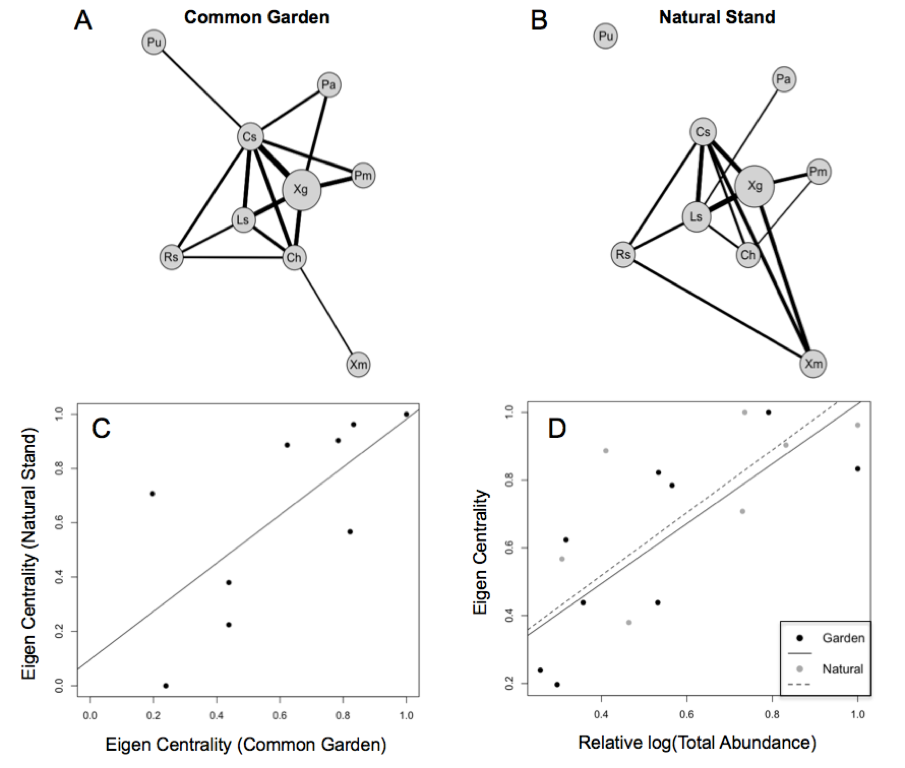
\includegraphics[width=\linewidth]{fig1}
%% \caption{Significant unipartite network structure was observed for
%%   epiphytic lichens on trees of known genotype in a common garden (ONC
%%   = Ogden Nature Center, Utah, USA) (A) and individual trees in a
%%   natural stand (Uintah, Utah, USA) (B) of the foundation species,
%%   \textit{Populus angustifolia}. Both networks are shown here with
%%   lichen species as nodes (see Methods for complete species names)
%%   scaled by the log of their total abundances and significant
%%   co-occurrence patterns between species shown as edges scaled by
%%   their log frequencies. The bivariate plot (C) shows the significant
%%   correlation in Eigen Centrality between the two networks. (D) The
%%   total abundance of lichen species was a significant driver of
%%   network structure for both networks.}
%% \label{fig:fig1}
%% \end{figure}

%% \begin{figure}[ht]
%% \centering
%% 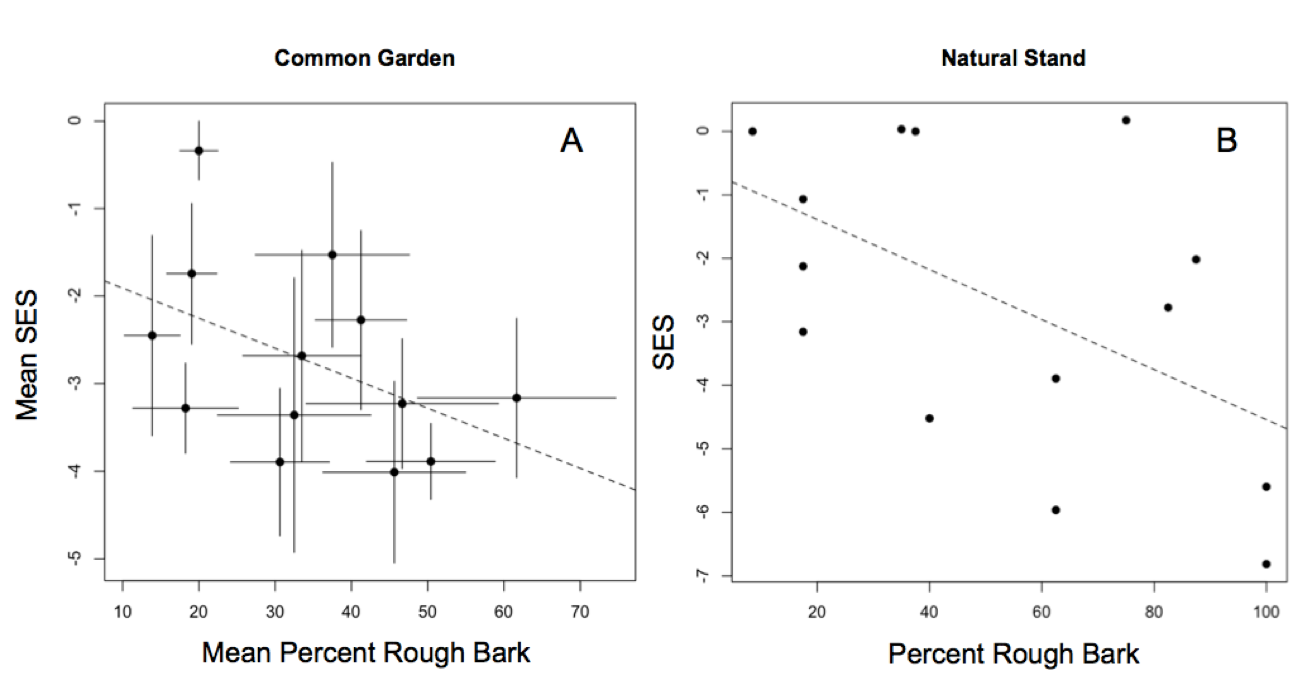
\includegraphics[width=\linewidth]{fig2}
%% \caption{Tree genotype influenced lichen co-occurrence patterns in the
%%   common garden and the natural stand through a genetically controlled
%%   tree trait. The lichen co-occurrence patterns were highly correlated
%%   with the genetically based phenotypic trait; bark roughness (i.e.,
%%   the percentage of textured bark), in both the common garden and
%%   natural stand. The scatterplot (A) shows the mean ($\pm$ 1 SE)
%%   percent rough bark (broadsense heritability, $H^2$ = 0.36, $\chi^2$
%%   = 9.214, \textit{p} = 0.002) and SES for each genotype for trees in
%%   the common garden with SES values becoming more negative (i.e.,
%%   species interactions increased), indicating stronger co-occurrence
%%   patterns, as bark roughness increases. The lichen communities on
%%   individual trees in the Unitah natural stand (B) displayed a similar
%%   pattern with the SES values becoming increasingly more negative on
%%   trees with more rough bark.}
%% \label{fig:fig2}
%% \end{figure}

\begin{figure}[ht]
\centering
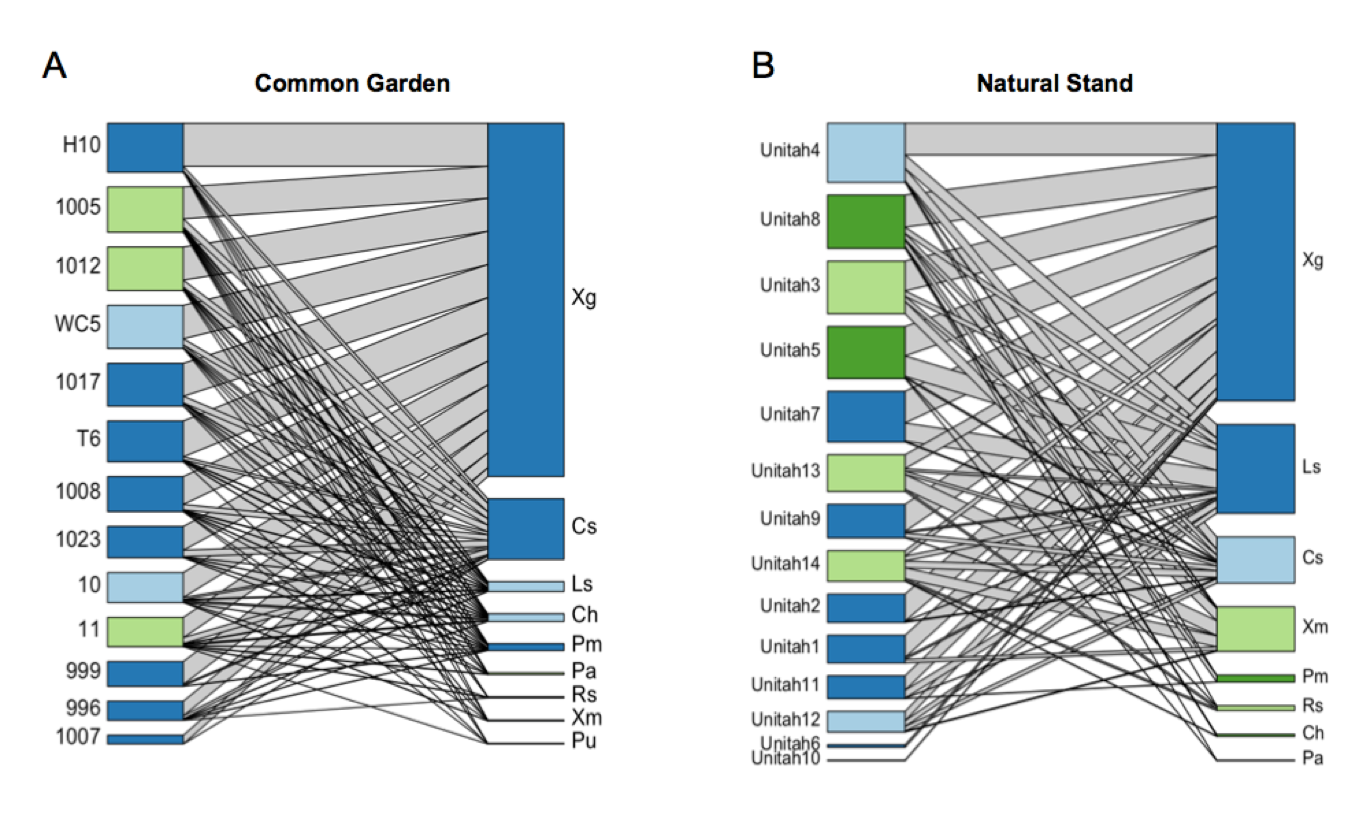
\includegraphics[width=\linewidth]{fig3}
\caption{Bipartite networks displayed significant modularity with
  modules comprised of both genotypes and species. The left most set
  of nodes shows tree genotypes (see Methods for genotype names) for
  the common garden (A) or individuals in the natural stand (B)
  connected to lichen species on the right. Both sets of nodes are
  scaled by their marginal totals (i.e., total observed individuals
  for tree nodes and total abundance for lichen species) and arranged
  by ascending totals from bottom to top. Node color shows the
  significant module membership for both trees and lichen species with
  module color having no direct relationship between the two networks,
  as modules were determined for each network independently.}
\label{fig:fig3}
\end{figure}

%% \begin{table}[ht]
%% \centering
%% \begin{tabular}{|l|l|l|}
%% \hline
%% Condition & n & p \\
%% \hline
%% A & 5 & 0.1 \\
%% \hline
%% B & 10 & 0.01 \\
%% \hline
%% \end{tabular}
%% \caption{\label{tab:example}Legend (350 words max). Example legend text.}
%% \end{table}

%% Figures and tables can be referenced in LaTeX using the ref command, e.g. Figure \ref{fig:stream} and Table \ref{tab:example}.

\end{document}
